\documentclass[9pt,technote]{IEEEtran}
\usepackage{fontspec}
\usepackage{graphicx}
\usepackage{float}
\usepackage{amssymb}
\usepackage{tabularx}
\usepackage{hyperref}
\usepackage{titling}
\usepackage{longtable}
\usepackage{acronym}
\usepackage{cite}
\usepackage{supertabular}
\usepackage[left=1.00in, right=1.00in, top=1.00in, bottom=1.00in]{geometry}
% \usepackage[page,toc,titletoc,title]{appendix}
\graphicspath{ {./images} }
\newfontfamily\dev[Script=Devanagari]{Nakula}

\linespread{1.3}
\setlength{\parskip}{5pt}
\setlength{\parindent}{0em}

\renewcommand\rmdefault{lmr}
\renewcommand\sfdefault{lmss}
\renewcommand\ttdefault{lmtt}

\newcommand{\code}[1]{\texttt{#1}}
\newcommand\tab[1][1cm]{\hspace*{#1}}

% \renewcommand{\bibname}{REFERENCES}
% \renewcommand{\contentsname}{TABLE OF CONTENTS}
% \renewcommand{\listfigurename}{LIST OF FIGURES}
% \renewcommand{\listtablename}{LIST OF TABLES}

\begin{document}

\pagenumbering{arabic}

\include{content}
% \section {Literature Review}
The dependency-based approach to grammar is much older than the relatively
recent phrase-structure or constituency grammars. While the notion of
constituency emerged during early 1900s, dependency grammar dates back to the
Indian grammarian Panini sometime between the 7th and 4th centuries BCE, as
well as the ancient Greek linguistic traditions\cite{stanfordLec}. The
formalization of dependency grammar was done by Chomsky(1956)\cite{chomsky}.
When a language can be formalized using Context Free Grammar, dependency
parsing can be done by using shift-reduce parsing algorithm initially developed
for analyzing programming languages, a work by Aho and Ullman\cite{ullman}. The
modern, deterministic, transition-based approach to dependency parsing was
pioneered by Nivre(2003)\cite{nivre1}. Neural method was first introduced by
Chen and Manning(2014)\cite{chen} the core concepts of which are still used by
the latest methods.
\newline
\newline
There are not as many works, however, done for South Asian languages like
Nepali. Although not as extensively as for English and Western languages, some
work has been done for Hindi/Tamil parsers \cite{tamilDep} and a very few for
Nepali.  Most of the works in Nepali are based on Paninian Grammar
\cite{paninianEng,yajnik1,yajnik2} and some extend that with rule based
framework \cite{balCompGrammar}. None of the Nepali parsers are data driven.
\\~\\
Almost all of the state-of-the art dependency parsers are neural based which
require lots of data. Following Chen and Manning\cite{chen}, Dyer et
al(2015)\cite{stackLstm} introduce a full vectorized representation of a
transition based parsing using stack-LSTMs which showed state-of-the-art
results.  Kiperwasser et al(2016)\cite{bistParser} also report rather simpler
feature representation for transition-based parser shown to be equally
effective to the existing best ones.
\\~\\
However, these methods alone are not feasible for low resource languages like
Nepali. There are works done in various directions to address this issue.
Traditional semi-supervised learning like self-training and co-training has
been used by Sagae et al \cite{semiSupervised1}. Following the line, more
robust system has been reported by Suzuki et al \cite{semiSupervised2}. Wenjuan
H. et al(2019)\cite{unsupervisedDP} even provided results with unsupervised
dependency parsing. However, their approach does not take into account the
dependency arc labels. In recent years, multilingual dependency parsing have
been shown to have even better performance \cite{malopa,multilingualCaseStudy}.
These models are particularly dependent on multilingual embeddings
\cite{multiEmbedding} and multilingual word clusters. Duc D. et
al(2021)\cite{vietnamese} used word alignments between English and Vietnamese
to use English treebank data for Vietnamese parsing.
\\~\\
Similar to \cite{malopa}, there are more recent approaches providing good
results for universal parsing. \cite{zero-shot} attempt zero-shot parsing based
on pretrained multilingual sentence representations. The first use of actual
language embeddings from typological databases is done in \cite{udapter} where
they propose adapter modules incorporated within BERT model to provide the
state-of-the-art universal parsing. To our knowledge, the latest of the methods
called STEPS parser tries to apply simple method for monolingual parsing
achieving the state-of-the-art.

% 
% \begin{table}[ht]
% \begin{center}
% \begin{tabular}{|c|c|c|}
%     \hline
%     \textbf{Authors} & \textbf{Year} & \textbf{Contribution} \\
%     \hline
%     Chomsky & 1956 & Formalization of dependency grammar \\
%     \hline
%     Nivre & 2003 & Modern Deterministic transition-based parsing \\
%     \hline
%     Bal Krishna Bal & 2004 & Structure of Nepali Grammar \\
%     \hline
%     Bal and Rupakheti & 2008 & Nepali Computational Grammar for Dependency Parsing \\
%     \hline
%     Dyer et al & 2015 & Neural transition-based parsing using stack-LSTMs \\
%     \hline
%     Ammar et al & 2016 & Multilingual parser based on Dyer et al \\
%     \hline
%     Kiperwasser et al & 2016 & Simple and accurate feature representations for Dependency Parsing \\
%     \hline
%     Lim et al & 2018 & Graph-based multilingual parsing in low-resource languages \\
%     \hline
%     Yajnik et al & 2019 & Dependency parsing using Linear Programming \\
%     \hline
%     Tran K. et al & 2019 & Zero-shot parsing using pretrained sentence representations \\
%     \hline
%     Ustun A. et al & 2020 & Language adapters for universal parsing \\
%     \hline
%     Duc D. et al & 2021 & Vietnamese dependency parsing using word order transformation \\
%     \hline
%     Grunewald S. et al & 2021 & Extensible and configurable Transformer-based parsing \\
%     \hline
% \end{tabular}
% \caption{Literature Review Summary}
% \label{table:literature_review}
% \end{center}
% \end{table}

% \chapter{Methodology}
This work is an extension of a wonderful paper \textit{`Applying Occam's Razor
to Transformer-Based Dependency Parsing: What works, What doesn't, and What is
really necessary'}\cite{steps-parser}. The parser is named STEPS(Stuttgart
Transformer based Extensible Parsing System) which indeed is a very flexible
parsing system. The idea is to use a multilingual parser which is trained on
multilingual BERT embeddings. Most of the work here follows the future
directions directed by the authors\cite{steps-parser} while combining some
concepts from UDapter\cite{udapter}. Finally, after all the experiments and
source language/size analysis, we parse Nepali sentences as a zero-shot case.

\begin{figure}[!h]
    \center
    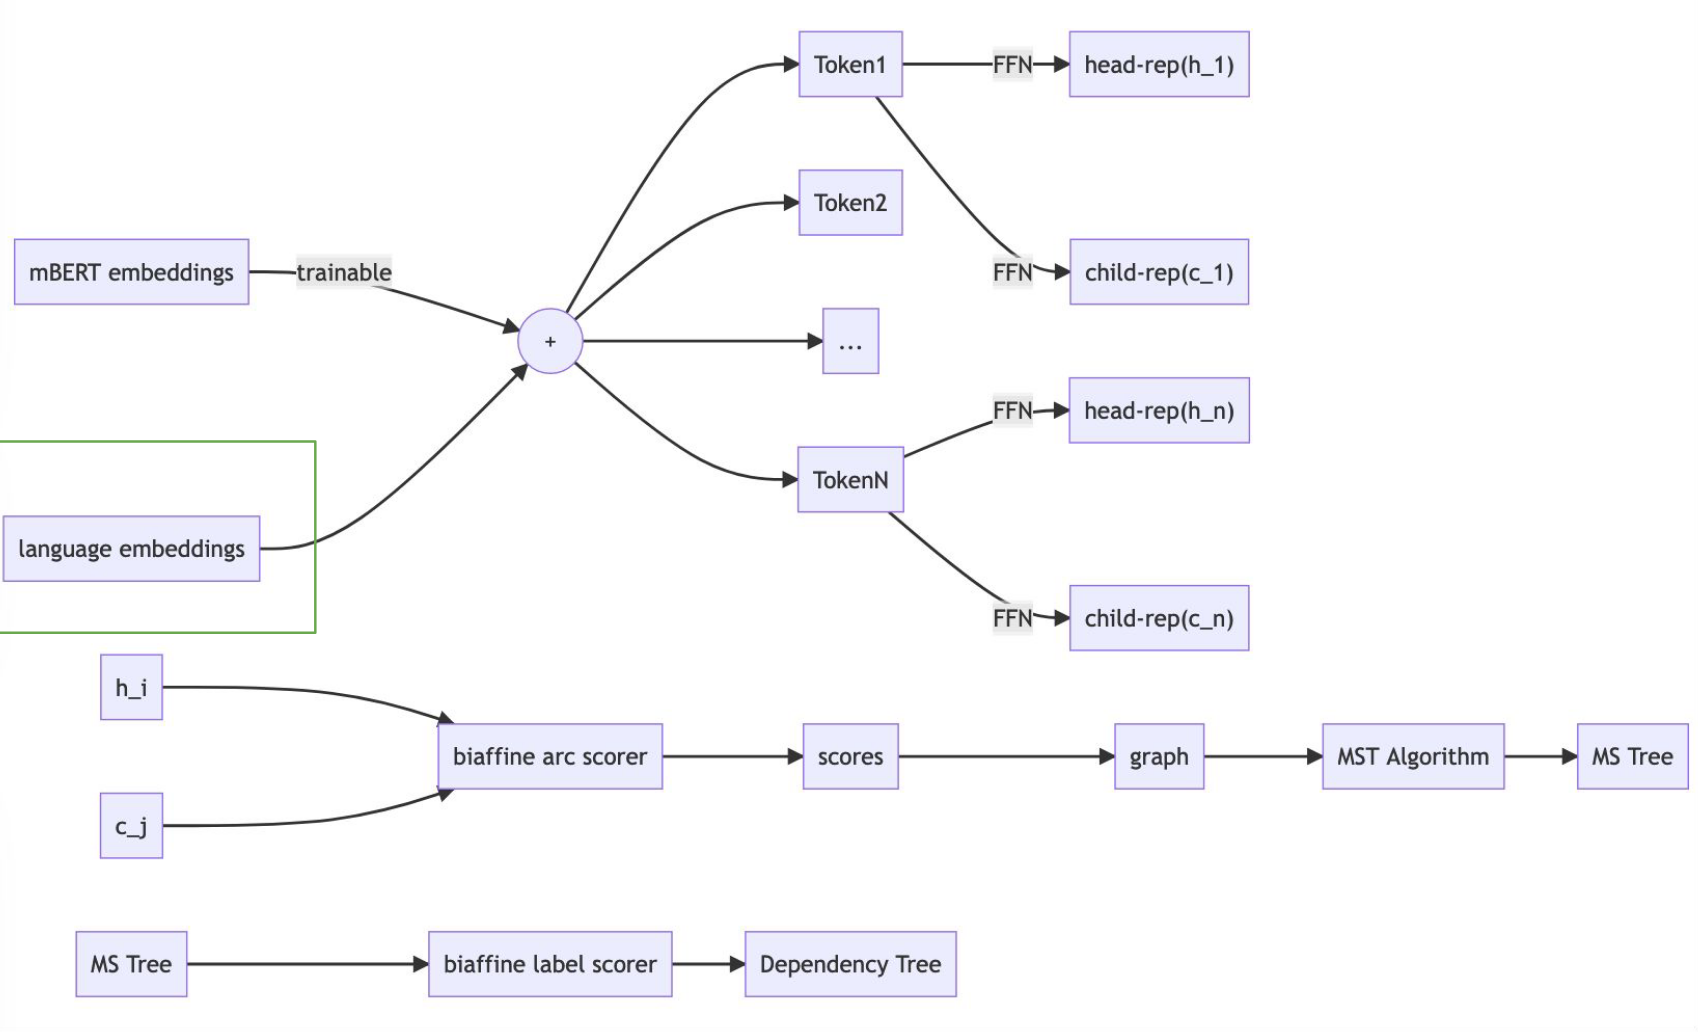
\includegraphics[scale=0.25]{images/Thesis_Architecture}
    \caption{System Architecture}
    \label{system_architecture}
\end{figure}

\section{Neural Graph-based Dependency Parsing}
This is the core idea behind the parser. We use neural graph-based parsing which works as follows:
\begin{itemize}
    \item[1.] For each word $w_i$, find scores for other words $w_j$ as the head of $w_i$ using some scoring function $S$ which will be a Biaffine classifier.
    \item[2.] This will give a set of edges which form a graph.
    \item[3.] Apply Maximum Spanning Tree Algorithm (CLE algorithm) to find the dependency arcs.
    \item[4.] For each arc, find the best scoring arc label, again using some scorer which will be a Biaffine classifier as well.
\end{itemize}

\section{System Architecture}
The latest advances in dependency parsing make use of contextualized language
embeddings like BERT, elmo and XLM-R. This work is an implementation of graph
based dependency parsing using pretrained BERT embeddings which are fine-tuned
as the model gets trained. The architecture is shown in figure
\ref{system_architecture} and the components are described below:

\subsection{mBERT Token Representations}
BERT is a contextualized Masked Language Model(MLM) that has proven to be very
effective for downstream tasks including dependency parsing. Since we are
aiming for transfer learning across various languages, monolingual BERT
embeddings are not adequete. Fortunately, multilingual BERT embeddings are
found for 104 languages, one of whom is Nepali. XLM-R have also shown to
provide better results but Nepali Embeddings are not available.  This makes
token representation using mBERT a natural choice for our task at hand.
The embeddings are fine tuned as the model is trained for dependency parsing.

\subsection{Language Embeddings}
Language embeddings are added at the later parts of the experiment. Since
different languages have different syntactic structures, training a
multilingual parser is a bit tricky. In our case, although Nepali and Hindi
have similar syntactic structures, English is quite different. And this results
in dependency annotations in Nepali or Hindi contradict to that in
English. Similar to \cite{udapter}, we use language embeddings from URIEL and
WALS databases provided by a library called \textit{lang2vec} which itself is
based on \cite{lang2vec}. However, we differ in that, while \cite{udapter} use
all of the 289 sparse features and train a linear model as a contextual
parameter generator, we reduce the dimensions to 18 to make them dense and
directly concat with the mBERT embeddings.

\subsection{Head and dependent representations}
The token representations(mBERT embeddings) obtained are passed to two
different Feed Forward Networks(FFNs) to get their representations as head and
as a child(dependent). Let $r_i$ be embedding vector for each token then,
$$h_i^{head} = FFN^{head}(r_i)$$
$$h_i^{dep} = FFN^{dep}(r_i)$$
Each of the input tokens will have two representations, one for head and another for child.

\subsection{Biaffine Classifier}
This is a scoring function defined as,
$$s_{i,j} = Biaff(h_i^{head}, h_j^{dep})$$
$$Biaff(x, y) = x^\top \textbf{U}y + \textbf{W}(x \oplus y) + \textbf{b}$$
where $\textbf{U}$, $\textbf{W}$ and $\textbf{b}$ are learned parameters and
$\oplus$ represents vector concatenation.

\subsection{Arc and label scoring}
This work uses \textbf{factorized} method for arc and label scoring in which,
arcs are scored first and based on the result, labels are scored. This can also
be done using \textbf{unfactorized} method but this gives no better result and
has more parameters.
\\~\\
Arc Scorer is a biaffine function which takes in every combination of
head-child tokens and assigns scores for each. Then a standard Maximum Spanning
Tree algorithm(generally CLE) is used to find relevant arcs.
\\~\\
Label scorer is also a biaffine function which takes in the arcs of the parsed
spanning tree and assigns corresponding labels.

\section{Evaluation and Validation}
\subsection{Evaluation Metrics}
The two widely used evaluation metrics for dependency parsing are:
\begin{itemize}
    \item \textbf{LAS}: Labeled Attachment Score is the percentage of correct head-modifier labeling among the expected relations.
    \item \textbf{UAS}: Unlabeled Attachment is the percentage of correct head-modifier relations identified among the expected relations.
\end{itemize}
As an example, consider the following ground truth of dependency relations
\begin{verbatim}
Index  Token      Head  Label
-----  -----      ----  -----
1      Book       0     root
2      me         1     dobj
3      a          4     det
4      flight     1     nobj
5      to         6     prep
6      Kathmandu  4     nmod
7      .          1     punct
\end{verbatim}
If the predicted relations are:
\\~\\
\begin{verbatim}
Index  Token      Head  Label  Head-correct?  Label-correct?
-----  -----      ----  -----  -------------  --------------
1      Book       0     root   yes            yes
2      me         1     dobj   yes            yes
3      a          4     amod*  yes            no
4      flight     1     nobj   yes            yes
5      to         5*    prep   no             yes
6      Kathmandu  4     aux*   yes            no
7      .          3*    punct  no             yes
\end{verbatim}
The LAS score is $\frac{correct-head-label-predictions}{total-relations} = \frac{3}{7} = 0.43$\\
The UAS score is $\frac{correct-head-predictions}{total-relations} = \frac{5}{7} = 0.71$

\section{Datasets}
Ideally, we would have a dataset from Universal Dependencies treebank.
Unfortunately, no such dataset exists as of now and thus 200 validation
sentences for Nepali had to be generated manually. Dataset of similar size has
been used by Lim et al(2018)\cite{multilingualCaseStudy} and in other zero shot
and low resource settings\cite{udapter}\cite{zero-shot} which led us to assume
that 200 should be a good enough validation size. A glimpse of what UD Treebank
dataset looks like is shown in Figure \ref{ud_structure}. The gold labels
defined in UD are show in Appendix \ref{ud_labels}.

\subsection{Training Datasets}
UD Treebank consists of rich collection of dependency parsing
annotations for various languages. Unfortunately, Nepali dependency
annotated datasets are not available in the treebank. Since this is a
transfer learning setup, we choose a subset of languages data in the treebank.
The languages are tabulated below in table \ref{table:dataset_summary}.
\begin{table}[!ht]
    \begin{center}
        \begin{tabular}{|l|l|c|}
            \hline
            \textbf{Language} & \textbf{Code} & \textbf{Dataset size} \\
            \hline
            Arabic & ar & 1500 \\
            \hline
            English & en & 1500 \\
            \hline
            Basque & eu & 1500 \\
            \hline
            Finnish & fi & 1500 \\
            \hline
            Hebrew & he & 1500 \\
            \hline
            Hindi & hi & 1500 \\
            \hline
            Italian & it & 1500 \\
            \hline
            Japanese & ja & 1500 \\
            \hline
            Korean & ko & 1500 \\
            \hline
            Russian & ru & 1500 \\
            \hline
            Swedish & sv & 1500 \\
            \hline
            Turkish & tr & 1500 \\
            \hline
            Chinese & zh & 1500 \\
            \hline
        \end{tabular}
        \caption{Dataset languages}
        \label{table:dataset_languages}
    \end{center}
\end{table}
These 13 languages were chosen as suggested in \cite{udapter}. The
languages consist of almost all the families of languages spoken in the world
so that the transfer learning becomes efficient.

\begin{figure}[!ht]
    \center
    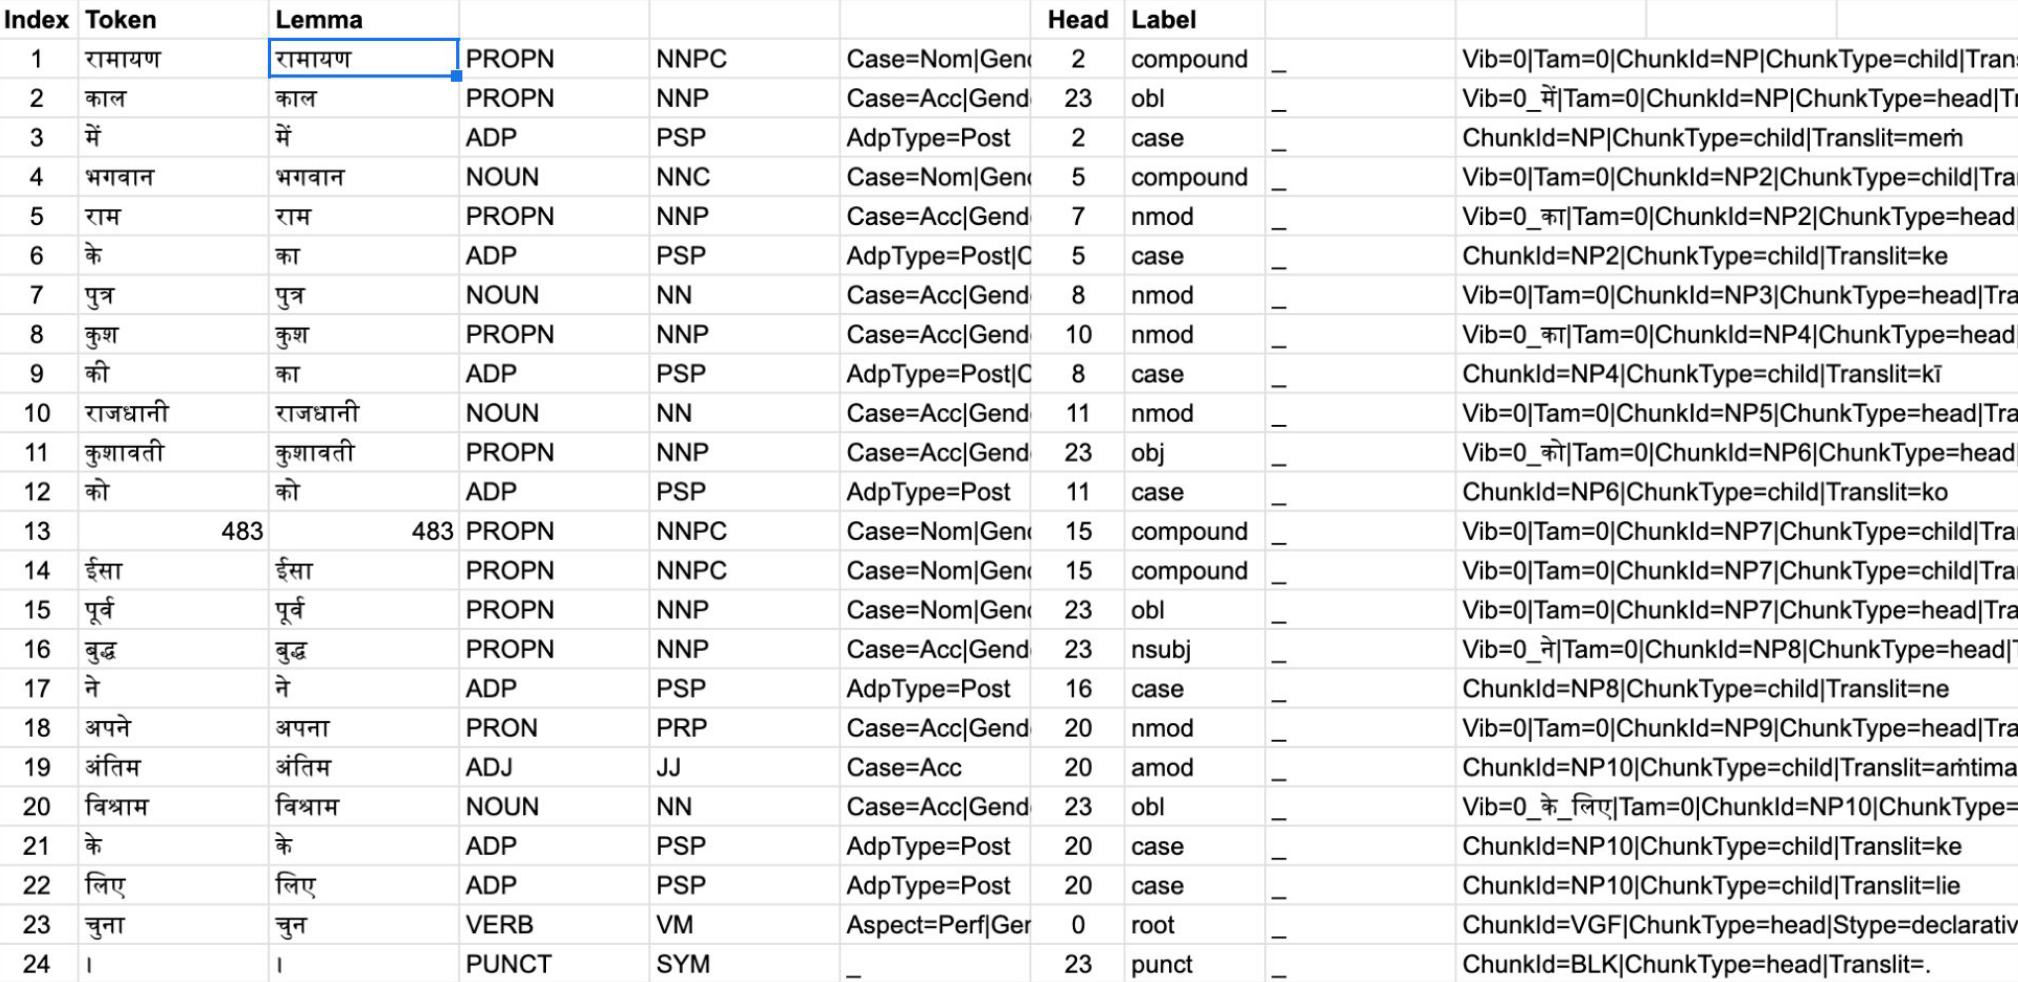
\includegraphics[trim={0 0 10cm 0},clip,scale=0.25]{images/ud_structure}
    \caption{Sample data in UD Treebank}
    \label{ud_structure}
\end{figure}

The dependency tree of an annotated sentence is shown in Figure \ref{dep_tree_example}
\begin{figure}[!ht]
    \center
    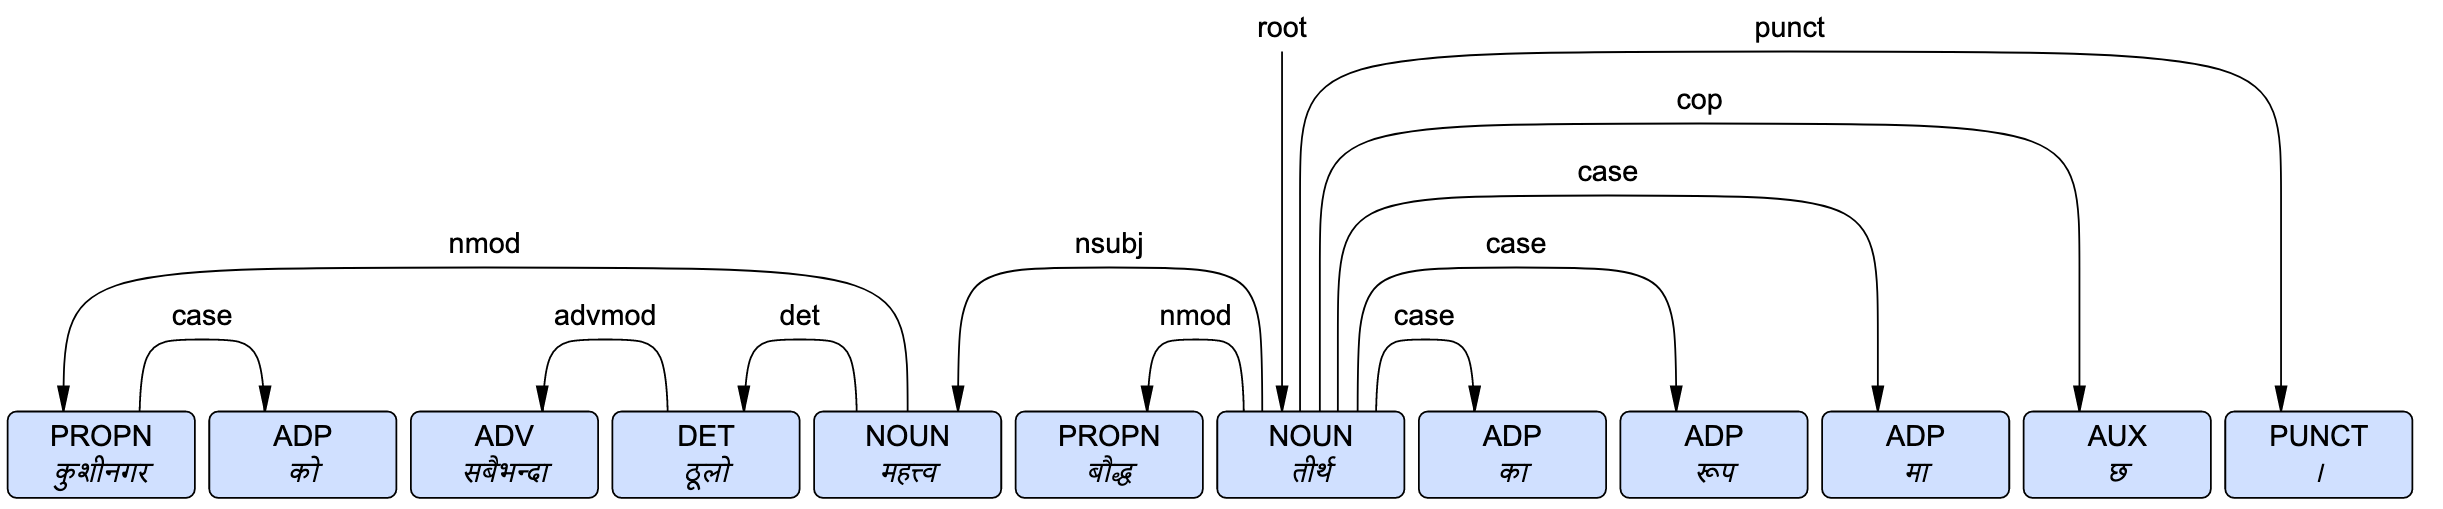
\includegraphics[scale=0.17]{images/nepali_dependency_parse}
    \caption{Dependency tree for a sentence in dataset}
    \label{dep_tree_example}
\end{figure}

\subsection{Validation Dataset}
As can be seen from Figure \ref{ud_structure} that manually creating dataset is
a long and tedious process even though only the columns \textit{Index, Token,
Head and Label} are required for dependency parsing. It is interesting to see
that since Hindi and Nepali language are very similar, if we have token-wise
translations of Hindi data, every other column can be reused except for the
\textit{Lemma} column. This work adopts the translation and alignment of Hindi
sentences in order to create an equivalent Nepali dataset. The following steps
were carried out while creating validation dataset:
\begin{itemize}
    \item[1.] Certain portion of the test dataset for Hindi was taken from the UD treebank. It is possible to align Hindi and Nepali while it's very hard for languages like English.
    \item[2.] It was preprocessed to obtain raw sentences. Each token was carefully preserved.
    \item[3.] The sentences were bulk translated by Google Translation and tokenized.
    \item[4.] However, the translations were not aligned. So a simple interactive tool was created that allowed manual corrections of wrong alignments.
    \item[5.] The results were verified by a fluent Hindi-Nepali speaker, whose summary is presented in Appendix \ref{translation}.
\end{itemize}
A summary of the dataset is shown below in Table \ref{table:dataset_summary}.
Incorrect translation summary is presented below in Table \ref{table:incorrect_summary}. Full enumeration of incorrect
translations is present in Appendix \ref{translation}.

\begin{table}[ht]
    \begin{center}
        \begin{tabular}{|l|c|}
            \hline
            Dataset Domain & Hindi News \\
            \hline
            Total Sentences & 200 \\
            \hline
            Total tokens & 3360 \\
            \hline
            Maximum tokens per sentence & 44 \\
            \hline
            Minimum tokens per sentence & 3 \\
            \hline
            Average tokens per sentence & 13 \\
            \hline
        \end{tabular}
        \caption{Dataset summary}
        \label{table:dataset_summary}
    \end{center}
\end{table}

\begin{table}
    \begin{center}
        \begin{tabular}{|l|c|}
            \hline
            Total Tokens & 3360 \\
            \hline
            Sentences with one or more errors & 31 \\
            \hline
            Incorrect token translations & 40 \\
            \hline
            Incorrect translation percentage & 1.19\% \\
            \hline
        \end{tabular}
        \caption{Incorrect translation summary}
        \label{table:incorrect_summary}
    \end{center}
\end{table}

\begin{figure}[!h]
    \center
    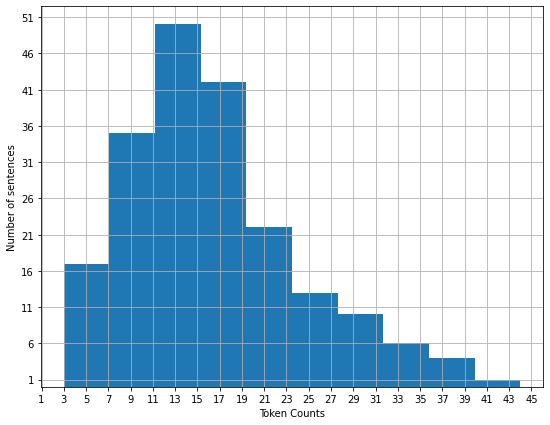
\includegraphics[scale=0.5]{images/dataset_histogram}
    \caption{Sentences - tokens count histogram}
    \label{tokens_count_histogram}
\end{figure}
Sample sentences are shown in Appendix \ref{dataset_summary_sample_appendix}.
\newpage

At first glance it might seem that having a 200 sentence tagged dataset might
not be sufficient even for validation/testing, let alone for training. However,
as we can see on the following table(parts copied from \cite{udapter}), on
average of only about 150 sentences are used for testing purposes.

\begin{table}[ht]
    \begin{center}
        \begin{tabular}{|c|c||c|}
            \hline
            \textbf{Language} & \textbf{Language Code} & \textbf{Dataset size} \\
            \hline
            Marathi & mr & 47 \\
            \hline
            Sanskrit & sa & 230 \\
            \hline
            Tamil & ta & 120 \\
            \hline
            Telugu & te & 146 \\
            \hline
            Bhojpuri & bho & 254 \\
            \hline
            \textbf{Average} & - & 159 \\
            \hline
        \end{tabular}
        \caption{Zero shot target dataset sizes}
        \label{table:zero_shot_dataset_sizes}
    \end{center}
\end{table}


\chapter{Results and Analysis}
\section{Experiments and Results}
All the datasets are used from UD treebank and the base implementation is by
\cite{steps-parser} which has been modified to include language embeddings as
well. We carry out series of experiments varying the languages, data sizes and language embeddings.
The following is the tabulation of experiments conducted and the results:
\begin{table}[ht]
    \begin{center}
        \scalebox{0.9}{
        \begin{tabular}{|c|c|c|c|c|c|}
            \hline
            \textbf{Exp. code} & \textbf{Languages} & \textbf{Dataset Size} & \textbf{Embeddings?} & \textbf{UAS} & \textbf{LAS} \\
            \hline
            rand & - & 0 & No & 12.75 & 3.48 \\
            \hline
            en2k & en & 2000 & No & 37.47 & 22.41 \\
            \hline
            en5k & en & 5000 & No & 38.30 & 22.68 \\
            \hline
            en & en & 10000 & No & 39.17 & 23.9 \\
            \hline
            hi & hi & 13000 & No & 50.74 & 39.32 \\
            \hline
            en\_hi & en,hi & 15000 & No & 41.31 & 32.67 \\
            \hline
            multi & multi & 18000 & No & 59.52 & 47.47 \\
            \hline
            multi\_np20 & \textbf{np},multi & 18020 & No & 71.22 & 59.97 \\
            \hline
            \textbf{multi\_np100} & \textbf{np},multi & 18100 & No & \textbf{76.98} & \textbf{67.29} \\
            \hline
            hi\_np20 & \textbf{np}, hi & 13020 & No & 69.59 & 60.79 \\
            \hline
            \textbf{hi\_np100} & \textbf{np},hi & 13100 & No & \textbf{80.73} & \textbf{72.67} \\
            \hline
            \textbf{np100} & \textbf{np} & 100 & No & \textbf{49.86} & \textbf{36.84} \\
            \hline
            \hline
            en2kem & en & 2000 & Yes & 32.43 & 23.07 \\
            \hline
            en5kem & en & 5000 & Yes & 32.66 & 22.31 \\
            \hline
            enem & en & 10000 & Yes & 35.79 & 24.2 \\
            \hline
            hiem & hi & 13000 & Yes & 52.18 & 40.71 \\
            \hline
            en\_hi\_em & en, hi & 15000 & Yes & 44.16 & 33.15 \\
            \hline
            multiem & multi & 18000 & Yes & 59.05 & 47.19 \\
            \hline
            \textbf{multi\_np20em} & \textbf{np},multi & 18020 & Yes & \textbf{71.22} & \textbf{59.43} \\
            \hline
        \end{tabular}
    }
        \caption{Experiments and results}
        \label{table:experiments_results}
    \end{center}
\end{table}
The \textbf{multi} languages are the languages mentioned in Table \ref{table:dataset_languages}.

\begin{figure}[!h]
    \center
    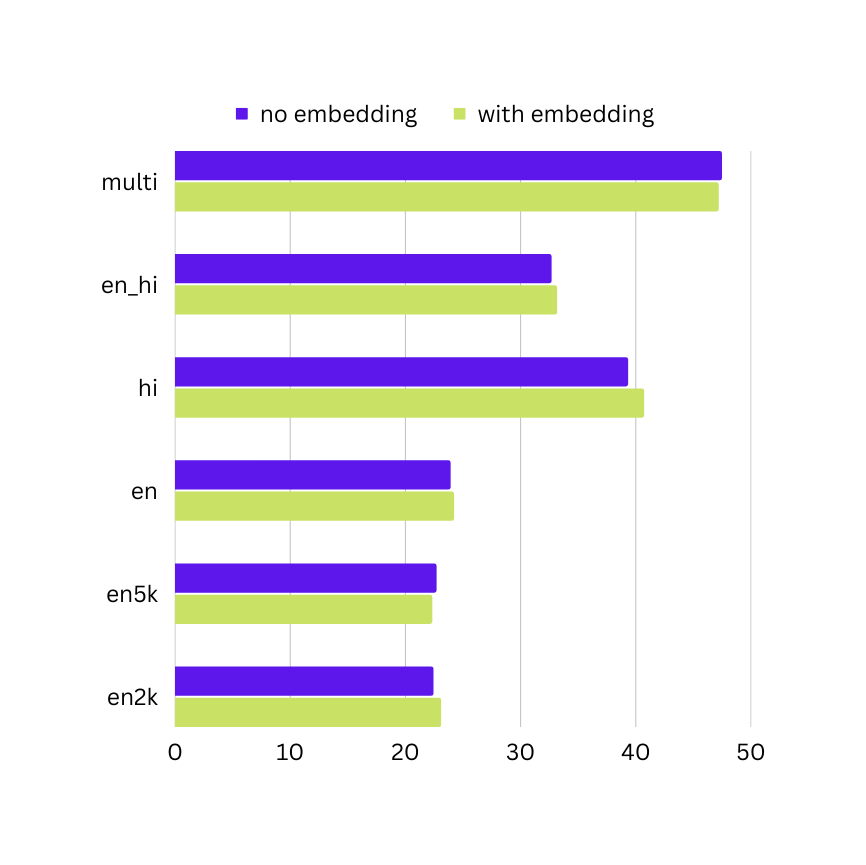
\includegraphics[scale=0.4]{images/results}
    \caption{Effects of language embeddings for zero-shot case}
    \label{results}
\end{figure}

\begin{figure}[!h]
    \center
    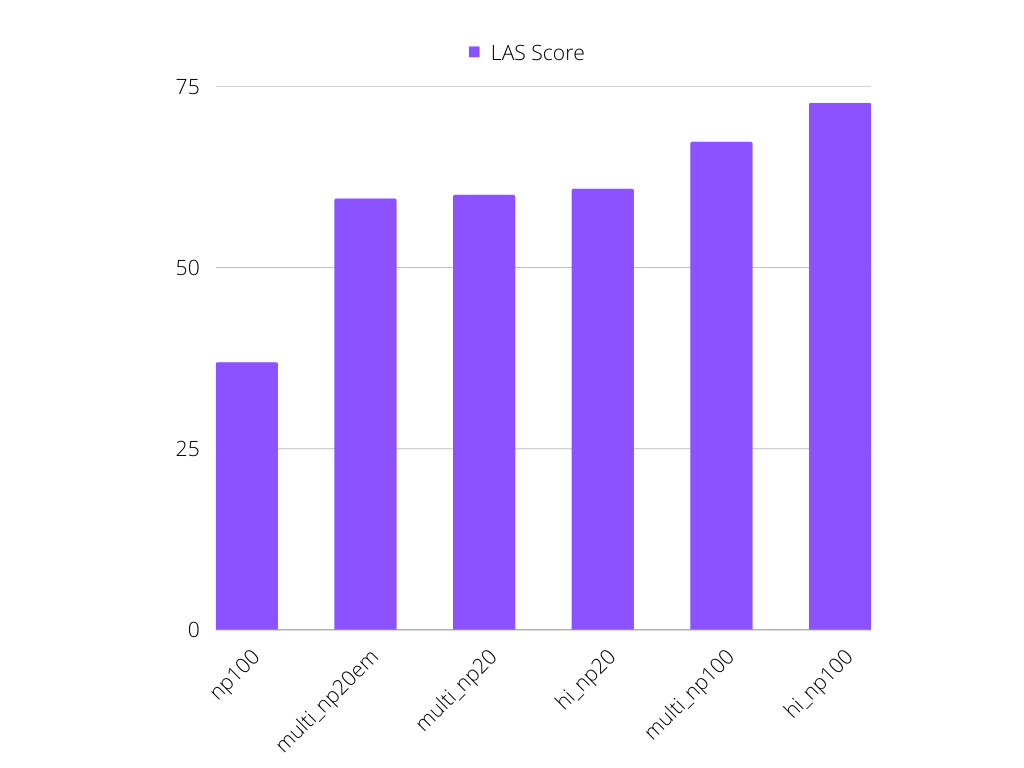
\includegraphics[scale=0.5]{images/fewshot_comparison}
    \caption{Comparison of fewshot experiments}
    \label{fewshot_comparison}
\end{figure}


The results are also summarized in Figure \ref{results}. So far, the best zero
shot LAS obtained is 47.38 for multi-source setup. We consider the previous
results on indic languages like Bhojpuri, Marathi, Sanskrit as the baseline.
Combining the results of \cite{zero-shot}\cite{udapter} for zero shot indic
languages like the highest average LAS obtained is \textbf{44.1}. Our result is
slightly better than the average. For the \textbf{few-shot} case where we used 20
Nepali sentences for training along with other languages, we have the highest
LAS score of \textbf{61.34} whereas with 100 Nepali sentences with
other languages, the score is 76.98. The result of parse on a sample sentence is shown in Figure \ref{img:sample_result1}

\section{Analysis}
The upper portion of table \ref{table:experiments_results} shows the results
when the original architecture by \cite{steps-parser} is used. The lower
portion shows the corresponding results when language embeddings is
incorporated in the architecture except for the random initialization. The
experiment codes are just for the shorthand names in graph.
\\~\\
Looking at the individual sections it is clear that some data is better than no
data and English as source underperforms Hindi as source. This is just a
verification of our intuition and underlying typographical relations of English
and Hindi with Nepali. Combining Hindi and English slightly degrades
performance in both sections which is also expected.
\\~\\
\textbf{Explanation of multi}\\
For multi language sources, we used the setup used by UDapter\cite{udapter}.
They use 13 different language-typologically diverse languages from over the
world. And it shows that the performance does increase significantly. Dataset
size has been made equal(around 12000 sentences) for each experiments that do
not explicitly mention size.
\\~\\
\textbf{Few-shot learning}\\
On the last rows of each section, the experiment names suffixed by
\textit{\_np*}, we present the results of few-shot learning where we used some
Nepali tagged sentences for training. As anyone would have anticipated, this
has increased the accuracy. It was not expected, however, that the difference
would be as big as 17\% even for just 20 Nepali sentences for training. And for
100 Nepali sentences in source training, the LAS scores obtained are 72.67\%.
This suggests that significant improvements in the scores can be obtained when
more Nepali sentences are used
as training.
\\~\\
\textbf{Effect of language embeddings}\\
Including language embeddings in the original architecture definitely shows
some improvements. The improvements are, however, not very significant. For the
case of multiple languages, the performance even decreases slightly. This might
be experimental error but we still have to investigate on this.
\\
The effect of concatenated language embeddings also seemed to be slightly
detrimental for few-shot cases. This perhaps indicates that for multi-source
training, mBERT already contains enough information about the languages
typology and concatenating language embeddings causes the effect of increased
training parameters to outweigh the increased accuracy due to language embeddings.
\\~\\
\textbf{Fully supervised learning}\\
We also evaluated the model when it was fully supervised by Nepali sentences
only.  For this, we split the 200 sentences as 100, 20 and 80 for training,
validation and testing respectively. The LAS score obtained is 36.84 which is
tabulated on the last row of upper experiments table. The score is clearly
better than using just English sentences for training. This is due to Nepali
language's dissimilarity with English. However the score is  slightly less than
training using Hindi only. This is because Nepali and Hindi are similar and
that the size of Hindi corpus is much bigger(~13k sentences) compared to
Nepali(100 sentences).
\\~\\
\textbf{Effect of Source Langauges}\\
For zero shot case, we can see from above table that using the 13
languages(multi) shows better score than when using Hindi only or Hindi and
English only. However for few-shot scenario, we can see that multi setup has
slightly less score than when using Hindi only(59.97 vs 60.79 for 20 sentences
and 67.29 vs 72.67 for 100 sentences). This suggests that when the target
language(Nepali) sentences are present in training, including typologically
dissimilar languages for training result in some level of noise for the parser.

\subsection*{Resources Used}
Majority of the experiments were run on AWS g4dn EC2 instance which has NVIDIA
T4 GPU.  Each experiment on average required around 13 hours. Some preliminary
runs were done on a workstation in LICT. The computation times for each
experiments are tabulated in Appendix \ref{experiments_time_appendix}.

\begin{figure}[!h]
    \center
    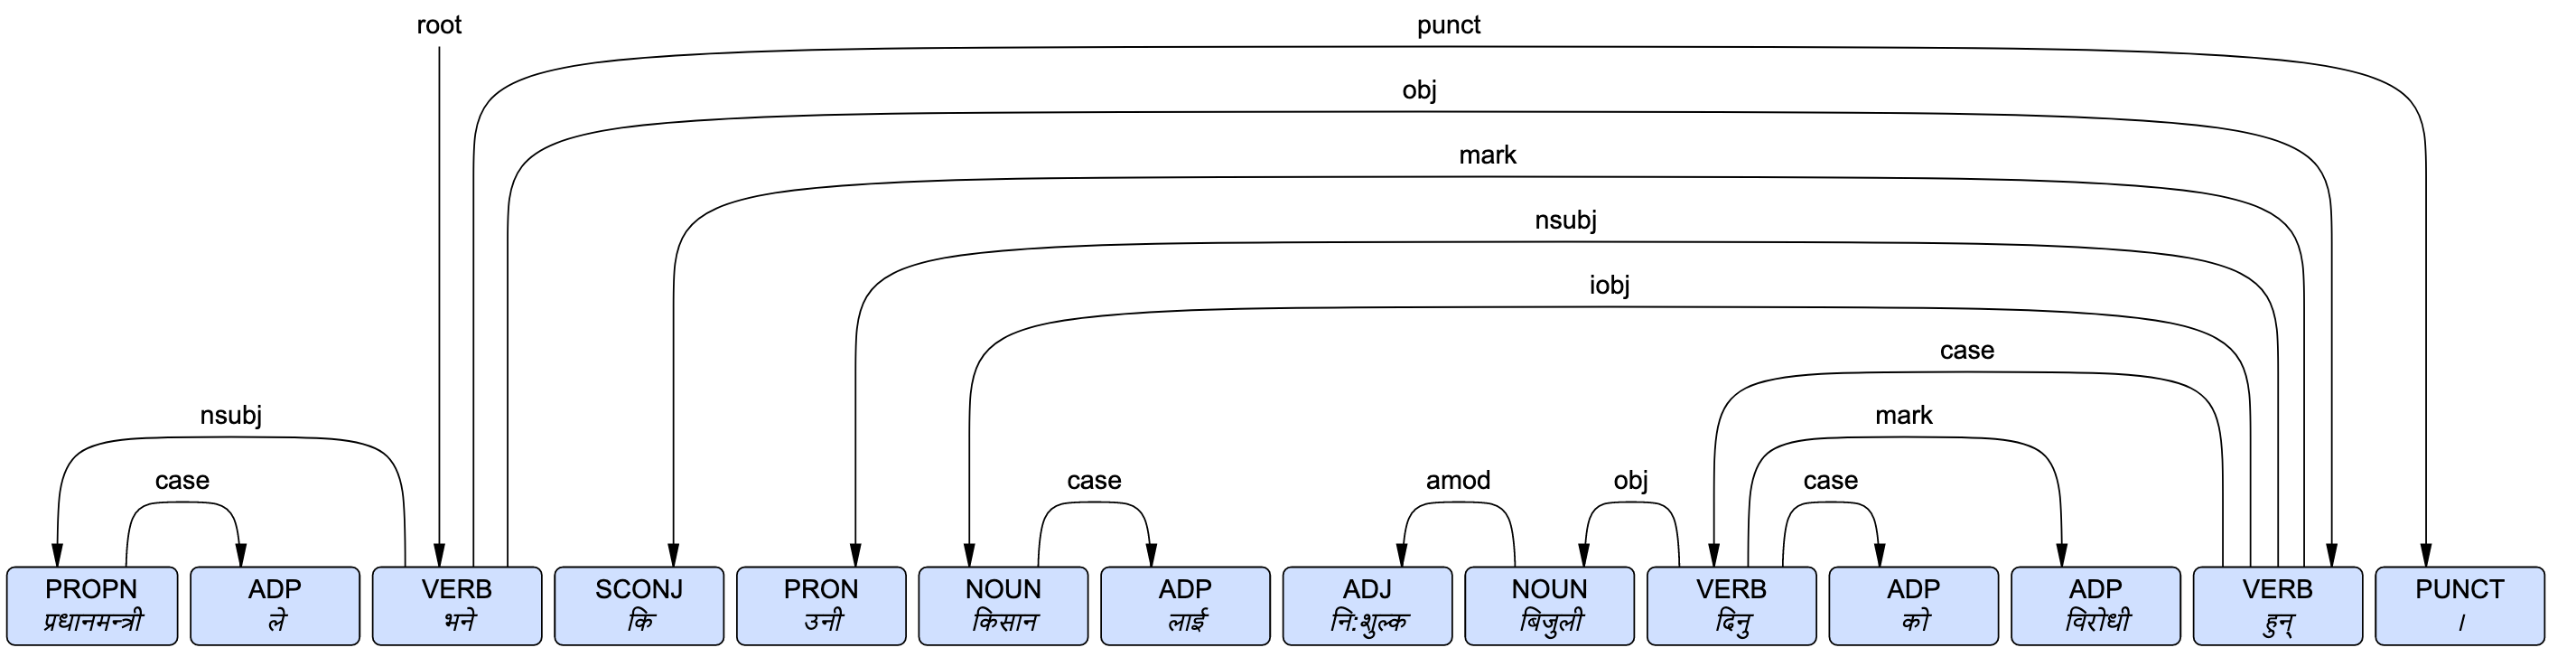
\includegraphics[scale=0.15]{images/sample_result}
    \caption{Sample parse of \dev{प्रधानमन्त्री ले भने कि उनी किसान लाई नि:शुल्क बिजुली दिनु को विरोधी हुन् ।}}
    \label{img:sample_result1}
\end{figure}
\chapter{Conclusions and Future Work}
The most important part of any machine learning system is the dataset.
In the case of Nepali dependency parsing, there have been no annotated
dataset. Manual annotation is a time consuming and technical task
especially in the case of Nepali dependency tags. In this work, the
task has been made easier by translating some parts of existing Hindi
treebank data and semi-automatically aligning the original Hindi and
translated Nepali sentences. Since Hindi and Nepali are similar, this
alignment allows to reuse the annotations for Hindi and saves a lot of
time. The dataset is also validated by a fluent Hindi-Nepali speaker.

After preparing the dataset, an existing state-of-the art Neural
Graph Parser was customized for transfer learning and a dependency
parser for Nepali was created and analyzed. A good baseline LAS score
of 72 has been achieved.

There are still spaces for improvement of the system. This work can be
extended in future to achieve the following:
\begin{itemize}
    \item [1.] Create more annotations.
    \item [2.] Experiment with source language variations.
    \item [3.] Fine tune BERT with language specific features.
\end{itemize}

% \chapter{Results}
Basic parsing of simple sentences have been carried out. Benchmarking dataset
is also created against which the metrics are evaluated.

\section{Sample Output}
\subsubsection{Sentence 1}
\dev{मोटो रामले खाना खाएर मोहनलाई झ्यालको किताब हातले दियो ।}
\\~\\
Pre-processed and POS-Tagged result:
\\~\\
(\dev{मोटो}, JJM) (\dev{राम}, NNP) (\dev{ले}, PLE) (\dev{खाना}, NN) (\dev{खाएर}, VBO)
(\dev{मोहन}, NNP) (\dev{लाई}, PLAI) (\dev{झ्याल}, NN) (\dev{को}, PKO) (\dev{किताब},
NN) (\dev{हात}, NN) (\dev{ले}, PLE) (\dev{दियो}, VBF) (\dev{।}, YF)
\\~\\
Initial chunking result:
\\~\\
\begin{table}[h]
\begin{center}
\begin{tabular}{|c|c|c|}
\hline
    \textbf{Chunk} & \textbf{Possible karak roles} & \textbf{CSP Variables} \\
    \hline 
(\dev{मोटो}, JJM) & [adjective] & \code{adjective\_0} \\ 
\hline 
(\dev{राम}, NNP) (\dev{ले}, PLE) & [karta, karan] & \code{karta\_1, karan\_1} \\ 
\hline 
(\dev{खाना}, NN) (\dev{खाएर}, VBO) & [vmod] & \code{vmod\_2} \\ 
\hline 
(\dev{मोहन}, NNP) (\dev{लाई}, PLAI) & [karma, sampradan] & \code{karma\_3, sampradan\_3} \\ 
\hline 
(\dev{झ्याल}, NN) (\dev{को}, PKO) & [sambandha] & \code{sambandha\_4} \\ 
\hline 
(\dev{किताब}, NN) & [karta, karma] & \code{karta\_5, karma\_5} \\ 
\hline 
(\dev{हात}, NN) (\dev{ले}, PLE) & [karta, karan] & \code{karta\_6, karan\_6} \\ 
\hline 
(\dev{दियो}, VBF) & [kriya] & \code{kriya\_7} \\ 
\hline 

\end{tabular}
\end{center}
\end{table}
\\~\\
Setting up constraints:
\\
\code{SEED}: (\dev{दिनु} \code{past}) \\
\code{
mitting non-LE karta for sakarmak kriya: karta\_5 == 0\\
SETTING mandatory karta: sum ['karta\_1', 'karta\_5', 'karta\_6'] == 1 \\
SETTING OPTIONAL karan: sum ['karan\_1', 'karan\_6']  <= 1 \\
SETTING OPTIONAL karma: sum ['karma\_3', 'karma\_5']  <= 1 \\
SETTING OPTIONAL sampradan: sum ['sampradan\_3']  <= 1 \\
Cooccuring  karta karan : karta\_1 - karan\_1 > 0\\
SETTING no karan before karta: karta\_1 - karan\_1 >= 0
SETTING single karta constraint: sum ['karta\_1', 'karta\_5', 'karta\_6']  <= 1\\
SETTING single karma constraint: sum ['karma\_3', 'karma\_5'] <= 1\\
}
Final constraint solved result:
\\~\\
\begin{figure}[h]
    \center
    \includegraphics[scale=0.8]{midterm_result_1}
    \caption{Dependency parse of sentence 1}
    \label{fig:result_1}
\end{figure}

\subsubsection{Sentence 2}
\dev{अहिले हाम्रा उत्पादन हरू मा अस्बेस्टस छैन ।}
\\~\\
Pre-processed and POS-Tagged result:
\\~\\
(\dev{अहिले}, RBO) (\dev{हाम्रा}, PP\$) (\dev{उत्पादन}, NN) (\dev{हरू}, HRU) (\dev{मा}, POP) (\dev{अस्बेस्टस}, NNP) (\dev{छैन}, VBX) (\dev{।}, YF)
\\~\\
Initial chunking result:
\\
\begin{table}[h]
\begin{center}
\begin{tabular}{|c|c|c|}
\hline
    \textbf{Chunk} & \textbf{Possible karak roles} & \textbf{CSP Variables} \\
    \hline
(\dev{अहिले}, RBO) & [vmod] & \code{vmod\_0} \\ 
\hline 
(\dev{हाम्रा}, PP\$) & [sambandha] & \code{sambandha\_1} \\ 
\hline 
(\dev{उत्पादन}, NN) (\dev{हरू}, HRU) (\dev{मा}, POP) & [adhikaran] & \code{adhikaran\_2} \\ 
\hline 
(\dev{अस्बेस्टस}, NNP) & [karta, karma] & \code{karta\_3, karma\_3} \\ 
\hline 
(\dev{छैन}, VBX) & [kriya] & \code{kriya\_4} \\ 
\hline 

\end{tabular}
\end{center}
\end{table}
\code{
SETTING OPTIONAL adhikaran: sum ['adhikaran\_2']  <= 1 \\
SETTING mandatory karta: sum ['karta\_3'] == 1 \\
SETTING OPTIONAL karma: sum ['karma\_3']  <= 1 \\
SETTING single karta constraint: sum ['karta\_3']  <= 1\\
SETTING single karma constraint: sum ['karma\_3'] <= 1\\
}
Final constraint solved result:
\\~\\
\begin{figure}[h]
    \center
    \includegraphics[scale=0.8]{midterm_result_2}
    \caption{Dependency parse of sentence 2}
    \label{fig:result_2}
\end{figure}

\subsubsection{Sentence 3}
\dev{बरू , यो निर्णय गर्न कम्पनी ले बजार लाई छोड्नेछ ।}
\\~\\
Pre-processed and POS-Tagged result:
\\~\\
(\dev{बरू}, CS) (\dev{,}, YM) (\dev{यो}, DUM) (\dev{निर्णय}, NN) (\dev{गर्न}, VBI) (\dev{कम्पनी}, NN) (\dev{ले}, PLE) (\dev{बजार}, NN) (\dev{लाई}, PLAI) (\dev{छोड्नेछ}, VBF)
\\~\\
Initial chunking result:
\\~\\
\begin{table}[h]
\begin{center}
\begin{tabular}{|c|c|c|}
\hline
    \textbf{Chunk} & \textbf{Possible karak roles} & \textbf{CSP Variables} \\
    \hline 
(\dev{बरू}, CS) & [unknown] & \code{unknown\_0} \\ 
\hline 
(\dev{,}, YM) & [unknown] & \code{unknown\_1} \\ 
\hline 
(\dev{यो}, DUM) & [adjective] & \code{adjective\_2} \\ 
\hline 
(\dev{निर्णय}, NN) (\dev{गर्न}, VBI) & [vmod] & \code{vmod\_3} \\ 
\hline 
(\dev{कम्पनी}, NN) (\dev{ले}, PLE) & [karta, karan] & \code{karta\_4, karan\_4} \\ 
\hline 
(\dev{बजार}, NN) (\dev{लाई}, PLAI) & [karma, sampradan] & \code{karma\_5, sampradan\_5} \\ 
\hline 
(\dev{छोड्नेछ}, VBF) & [kriya] & \code{kriya\_6} \\ 
\hline 

\end{tabular}
\end{center}
\end{table}
\\~\\
Setting up constraints:
\\
\code{SEED}: (\dev{छोड्नु} future ) \\
\code{
SETTING mandatory karta: sum ['karta\_4'] == 1 \\
SETTING OPTIONAL karan: sum ['karan\_4']  <= 1 \\
SETTING OPTIONAL karma: sum ['karma\_5']  <= 1 \\
SETTING OPTIONAL sampradan: sum ['sampradan\_5']  <= 1 \\
SETTING no karan before karta: karta\_4 - karan\_4 >= 0
SETTING single karta constraint: sum ['karta\_4']  <= 1\\
SETTING single karma constraint: sum ['karma\_5'] <= 1\\
}
Final constraint solved result:
\\~\\
\begin{figure}[h]
    \center
    \includegraphics[scale=0.8]{midterm_result_3}
    \caption{Dependency parse of sentence 3}
    \label{fig:result_3}
\end{figure}

\subsubsection{Sentence 4}
\dev{साउदर्न अप्टिकल को बिक्री कार्यक्रम को एउटा भाग हो ।}
\\~\\
Pre-processed and POS-Tagged result:
\\~\\
(\dev{साउदर्न}, NNP) (\dev{अप्टिकल}, NNP) (\dev{को}, PKO) (\dev{बिक्री}, NN) (\dev{कार्यक्रम}, NN) (\dev{को}, PKO) (\dev{एउटा}, CL) (\dev{भाग}, NN) (\dev{हो}, VBX) (\dev{।}, YF)
\\~\\
Initial chunking result:
\\~\\
\begin{table}
\begin{center}
\begin{tabular}{|c|c|c|}
\hline
    \textbf{Chunk} & \textbf{Possible karak roles} & \textbf{CSP Variables} \\
    \hline 
(\dev{साउदर्न}, NNP) (\dev{अप्टिकल}, NNP) (\dev{को}, PKO) & [sambandha] & \code{sambandha\_0} \\ 
\hline 
(\dev{बिक्री}, NN) & [karta, karma] & \code{karta\_1, karma\_1} \\ 
\hline 
(\dev{कार्यक्रम}, NN) (\dev{को}, PKO) & [sambandha] & \code{sambandha\_2} \\ 
\hline 
(\dev{एउटा}, CL) & [adjective] & \code{adjective\_3} \\ 
\hline 
(\dev{भाग}, NN) & [karta, karma] & \code{karta\_4, karma\_4} \\ 
\hline 
(\dev{हो}, VBX) & [kriya] & \code{kriya\_5} \\ 
\hline 
\end{tabular}
\end{center}
\end{table}
\\~\\
Setting up constraints:
\\
\code{
SETTING mandatory karta: sum ['karta\_1', 'karta\_4'] == 1 \\
SETTING OPTIONAL karma: sum ['karma\_1', 'karma\_4']  <= 1 \\
Cooccuring  karta karma : karta\_1 - karma\_1 > 0\\
SETTING single karta constraint: sum ['karta\_1', 'karta\_4']  <= 1\\
SETTING single karma constraint: sum ['karma\_1', 'karma\_4'] <= 1\\
}
Final constraint solved result:
\\~\\
\begin{figure}[h]
    \center
    \includegraphics[scale=0.8]{midterm_result_4}
    \caption{Dependency parse of sentence 4}
    \label{fig:result_4}
\end{figure}

\normalfont

\section{Summary}
The tagged dataset contains 62 sentences tagged using a tagging user interface.
The data is summarized below.
\begin{table}[h]
    \begin{center}
        \begin{tabular}{|c|c|}
            \hline
            \textbf{Data} & \textbf{Count} \\
            \hline
            Sentences & 62 \\
            \hline
            Words/Tokens & 512 \\
            \hline
            Attachments/Links & 387 \\
            \hline
        \end{tabular}
    \end{center}
    \caption{Data Summary}
    \label{table:data_summary}
\end{table}
Formulating as a Constraint Satisfaction Problem, a sentence is either parsed
or not at all because of the discrete nature of CSP variables. The LAS  and UAS are calculated for
only the sentences that had a solution \textendash { } about 50 sentences.
Chunking has not been evaluated as it will be indicated by LAS and UAS.
The results are tabulated below.
\begin{table}[h]
    \begin{center}
        \begin{tabular}{|c|c|}
            \hline
            \textbf{Metric} & \textbf{Accuracy} \\
            \hline
            LAS & 0.542 \\
            \hline
            UAS & 0.628 \\
            \hline
            POS Tagging & 0.96 \\
            \hline
            Solution Accuracy & 0.758 \\
            \hline
        \end{tabular}
    \end{center}
    \caption{Accuracy result}
    \label{table:accuracy_result}
\end{table}

\section{Error Analysis}
The POS Tagging accuracy seems to be excellent due to the use of the reliable
TnT Tagger. The LAS and UAS are not very exciting. Although close to 0.5, it is
important to note that these are still much better than random assignments.
This is because, a sentence of average length 10 has 9 links among the words
which has approximately ${}_{9}C_{2}$ possible combinations and each link can have about 10
labels. Thus, the probability for correctly finding and labeling links for a
random tagger is much less than 0.5.
\\~\\
The existing errors are mainly due to the following:
\begin{itemize}
    \item[a.] Presence of multi-word noun phrases. For example: \dev{मेनफ्रेम कम्प्युटरहरु}
        \normalfont
        is chunked as two nouns instead of single entity. When this
        chunking is used, the CSP can't find solutions because both of these
        terms are treated as \textit{karta}.
    \item[b.] Incomplete or imperfect chunk rules. There are still more chunk
        rules to be discovered and added. For example: a rule for
        \textit{sampradan} \textendash { } \dev{- को/का लागि}
        \normalfont
        is not yet incorporated.
        Similarly, chunking is not working well for phrases containing an
        adjective(JJ) and infinitive(VBI) e.g. \dev{उपस्थित हुन}
        \normalfont
    \item[c.] Some of the verb modifier chunks are also not in the rule. For
        example, \dev{२० वर्ष सम्म}
        \normalfont
   \itemsep0em
    \item[d.] Some verb identifiers are chunked incorrectly. For example,
        \dev{भने छैनन्}
        \normalfont
        is chunked as a verb phrase but in fact it consists of an
        adverb and verb. The rule set needs to include such constructs as well.
    \item[e.] The dataset consists of substantial amount of complex sentences
        like quotations and conjunctions. There are no rules for such sentences
        yet.
\end{itemize}

% \newpage
% \chapter{Limitations}
The following are the current limitations of the parser:
\begin{itemize}
    \item[1.] It is heavily dependent on the POS Tagger. If the POS tagged results are poor, the parser has high chance of failing.
    \item[2.] The POS tagger has also been trained using limited data(just about 90,000 words). So, it has difficulties coping with new words.
    \item[3.] Some entities are represented by multiple words. For example,
        is very difficult by just looking at POS tags to discern if the
        consecutive \code{NN}s refer to single entity or two.
    \item[4.] Only simple sentences are parsed. The parser has yet to parse passive sentences, questions imperatives and other complex forms.
    \item[7.] The labels partially conform with the Universal Dependency labels. A
        mapping and transformation to UD labels needs to be done.
\end{itemize}



% \newpage
% \chapter{Conclusions and Future Work}
This project shows an experimentation with rule-based system for dependency
parsing based on Paninian framework. The following are the conclusions:
\begin{itemize}
    \item LAS of 0.542 and UAS of 0.628 have been achieved against the dataset of 62 sentences tagged manually.
    \item Due to lack of dependency dataset, corpus based methods are not yet possible.
    \item Natural language, especially Nepali, has many constructs and thus requires lots of rules to address different language forms.
    \item The parser is still to handle quotations, conjunctions and reported speeches.
    \item The parser can also be extended to create knowledge graph and information retrieval systems.
\end{itemize}

\subsubsection{Future Work/Scope for Thesis}
This project can be extended in the following ways for thesis:
\begin{itemize}
    \item[1.] Add more rules and handle more complex sentences.
    \item[2.] Create a larger dataset in a semi-automated way - using the results from the parser and modifying where needed.
    \item[3.] Use the state-of-the-art BiLSTM models for dependency parsing using the created dataset.
\end{itemize}



% \newpage

\begin{appendices}
\include{appendix}
% \chapter{Annotated sentences samples} \label{dataset_summary_sample_appendix}

The following are 100 out of 200 annotated sentences created. Note that the
underscores(\_) represents the dummy token for the tokens that could not be perfectly aligned. For example:
\begin{itemize}
    \item For verbs like: \dev{करता है} whose translation is \dev{गर्दछ \_}
    \item For adjective phrases like: \dev{बड़ा सा} whose translation is \dev{ठुलो \_}
\end{itemize}


The following consist of a Hindi sentence, translated Nepali sentence and the
corresponding annotated data. And the tabulation of annotations is shown in
Table \ref{table:sample_annotation1}\\
\textbf{Hindi:} \dev{कुशीनगर का महत्‍व महापरिनिर्वाण मंदिर से है ।}\\
\textbf{Nepali:} \dev{कुशीनगर को महत्व महापरिनिर्वाण मन्दिर बाट हो ।}\\
\begin{table}[ht]
    \begin{center}
        \scalebox{0.8}{
            \begin{tabular}{|c|c|c|c|c|c|c|c|}
            \hline
            \textbf{\tiny{Index}} & \textbf{\tiny{Token}} & \textbf{\tiny{Lemma}} & \textbf{\tiny{UPOS}} & \textbf{\tiny{XPOS}} & \textbf{\tiny{Feats}} & \textbf{\tiny{Head}} & \textbf{\tiny{Label}} \\
            \hline
            1 & \scriptsize{\dev{कुशीनगर}} & \scriptsize{\dev{कुशीनगर}} & \scriptsize{PROPN} & \scriptsize{NNP} & \tiny{Case=Acc|Gender=Masc|Number=Sing|Person=3} & 3 & \scriptsize{nmod} \\
            \hline
            2 & \scriptsize{\dev{को}} & \scriptsize{\dev{का}} & \scriptsize{ADP} & \scriptsize{PSP} & \tiny{AdpType=Post|Case=Nom|Gender=Masc|Number=Sing} & 1 & \scriptsize{case} \\
            \hline
            3 & \scriptsize{\dev{महत्व}} & \scriptsize{\dev{महत्व}} & \scriptsize{NOUN} & \scriptsize{NN} & \tiny{Case=Nom|Gender=Masc|Number=Sing|Person=3} & 5 & \scriptsize{nsubj} \\
            \hline
            4 & \scriptsize{\dev{महापरिनिर्वाण}} & \scriptsize{\dev{महापरिनिर्वाण}} & \scriptsize{PROPN} & \scriptsize{NNPC} & \tiny{Case=Nom|Gender=Masc|Number=Sing|Person=3} & 5 & \scriptsize{compound} \\
            \hline
            5 & \scriptsize{\dev{मन्दिर}} & \scriptsize{\dev{मंदिर}} & \scriptsize{PROPN} & \scriptsize{NNP} & \tiny{Case=Acc|Gender=Masc|Number=Sing|Person=3} & 0 & \scriptsize{root} \\
            \hline
            6 & \scriptsize{\dev{बाट}} & \scriptsize{\dev{से}} & \scriptsize{ADP} & \scriptsize{PSP} & \tiny{AdpType=Post} & 5 & \scriptsize{case} \\
            \hline
            7 & \scriptsize{\dev{हो}} & \scriptsize{\dev{है}} & \scriptsize{AUX} & \scriptsize{VM} & \tiny{Mood=Ind|Number=Sing|Person=3|Tense=Pres|VerbForm=Fin} & 5 & \scriptsize{cop} \\
            \hline
            8 & \scriptsize{\dev{।}} & \scriptsize{\dev{।}} & \scriptsize{PUNCT} & \scriptsize{SYM} & \tiny{\_} & 5 & \scriptsize{punct} \\
            \hline
        \end{tabular}
        \caption{Annotation for Sample sentence 1}
        \label{table:sample_annotation1}
    \end{center}
\end{table}


\subsubsection{Sentences}
Some of the translated nepali sentences are:
\begin{itemize}
    \item[1.] \dev{रामायण काल मा भगवान राम का छोरा कुश को राजधानी कुशावती लाई 483 ईसा पूर्व बुद्ध ले आफ्नो अन्तिम विश्राम को लागि चुने ।}

    \item[2.] \dev{मल्लहरू को राजधानी भए को कारण प्राचीनकाल मा यस स्थान को ठूलो महत्व थियो ।}

    \item[3.]\dev{हिन्दू राजाहरू को काल मा चीन बाट ह्युएन त्साङ , फाहियन र इट्सिङ ले आफ्नो यात्रा विवरण मा यस ठाउँ को महिमा को वर्णन गरेका छन् ।}

    \item[4.]\dev{कुशीनगर को सबैभन्दा ठूलो महत्त्व बौद्ध तीर्थ का रूप मा छ ।}

    \item[5.]\dev{कुशीनगर को सीमा मा प्रवेश गर्दा बित्तिकै भव्य प्रवेशद्वार तपाईंको स्वागत गर्दछ \_ ।}

    \item[6.]\dev{कुशीनगर को महत्व महापरिनिर्वाण मन्दिर बाट हो ।}

    \item[7.]\dev{यस मन्दिर को वास्तुकला अजन्ता को गुफा बाट प्रेरित छ ।}

    \item[8.]\dev{यो मन्दिर त्यही ठाउँ मा निर्माण गरिएको हो , जहाँ बाट यो मूर्ति निकालिएको \_ थियो ।}

    \item[9.]\dev{मन्दिर को पूर्व भाग मा एउटा स्तूप छ ।}

    \item[10.]\dev{यहाँ \_ भगवान बुद्ध को अंतिम दाहसंस्कार गरिएको \_ थियो ।}

    \item[11.]\dev{मूर्ति पनि अजन्ता को भगवान बुद्ध को महापरिनिर्वाण मूर्ति को प्रतिकृति हो ।}

    \item[12.]\dev{वैसे मूर्ति को अवधि अजन्ता भन्दा पहिले को हो ।}

    \item[13.]\dev{यस मन्दिर को वरिपरि धेरै विहारहरू ( जहाँ बौद्ध भिक्षुहरू बस्ने गर्दथे \_ ) र चैत्यहरू ( जहाँ भिक्षुहरू पूजा गर्थे \_ वा ध्यान लगाउँथे \_ ) भग्नावशेषहरू र खंडहर रहेका छन् जुन अशोककालीन भन्ने गरिन्छ \_ ।}
\end{itemize}


% \chapter{Universal Dependencies Labels} \label{ud_labels}
\begin{longtable}{| p{.20\textwidth} | p{.80\textwidth} |}
            \hline
            \textbf{Label} & \textbf{Meaning} \\
            \hline
            acl & Clausal Modifier Of Noun (Adnominal Clause) \\
            \hline
            advcl & Adverbial Clause Modifier \\
            \hline
            advmod & Adverbial Modifier \\
            \hline
            amod & Adjectival Modifier \\
            \hline
            appos & Appositional Modifier \\
            \hline
            aux & Auxiliary \\
            \hline
            case & Case Marking \\
            \hline
            cc & Coordinating Conjunction \\
            \hline
            ccomp & Clausal Complement \\
            \hline
            clf & Classifier \\
            \hline
            compound & Compound \\
            \hline
            conj & Conjunct \\
            \hline
            cop & Copula \\
            \hline
            csubj & Clausal Subject \\
            \hline
            dep & Unspecified Dependency \\
            \hline
            det & Determiner \\
            \hline
            discourse & Discourse Element \\
            \hline
            dislocated & Dislocated Elements \\
            \hline
            expl & Expletive \\
            \hline
            fixed & Fixed Multiword Expression \\
            \hline
            flat & Flat Multiword Expression \\
            \hline
            goeswith & Goes With \\
            \hline
            iobj & Indirect Object \\
            \hline
            list & List \\
            \hline
            mark & Marker \\
            \hline
            nmod & Nominal Modifier \\
            \hline
            nsubj & Nominal Subject \\
            \hline
            nummod & Numeric Modifier \\
            \hline
            obj & Object \\
            \hline
            obl & Oblique Nominal \\
            \hline
            orphan & Orphan \\
            \hline
            parataxis & Parataxis \\
            \hline
            punct & Punctuation \\
            \hline
            reparandum & Overridden Disfluency \\
            \hline
            root & Root \\
            \hline
            vocative & Vocative \\
            \hline
            xcomp & Open Clausal Complement \\
            \hline
        \caption{Arc labels and the meanings}
        \label{table:label_meanings}
\end{longtable}

\chapter{Translation Information} \label{translation}
Some information about the human validator is tabulated below:
\begin{table}[ht]
    \begin{center}
        \begin{tabular}{|l|c|}
            \hline
            Age & 26 \\
            \hline
            Education & M.Sc. \\
            \hline
            Mother tongue & Nepali \\
            \hline
            Hindi proficiency & Fluent \\
            \hline
        \end{tabular}
        \caption{Validator Description}
        \label{table:validator_description}
    \end{center}
\end{table}

The following are all the errors reported by the validator: \\
\dev{ महानियंत्रक -> नियन्त्रक }\\
\dev{ लेखा -> महालेखा }\\
\dev{ पर -> को }\\
\dev{ उपाध्यक्ष -> उपसभामुख }\\
\dev{ किया -> गरेको }\\
\dev{ सत्ता -> अख्तियार }\\
\dev{ 19,401 -> 233 }\\
\dev{ आदिवासी -> जनजाति }\\
\dev{ उनकी -> आफ्नो }\\
\dev{ से -> ले }\\
\dev{ पश्चिमी -> पश्चिमाञ्चल }\\
\dev{ वह -> उनी }\\
\dev{ के -> को }\\
\dev{ आया -> आए }\\
\dev{ तरह -> तरिक }\\
\dev{ जीडीपी -> उत्पादन }\\
\dev{ २६.४ -> 26 }\\
\dev{ उपाध्यक्ष -> उपराष्ट्रपति }\\
\dev{ राजद -> आरजेडी }\\
\dev{ अध्यक्ष -> राष्ट्रपति }\\
\dev{ सामने -> नजिक }\\
\dev{ तो -> त्यसोभए }\\
\dev{ वाली -> वल }\\
\dev{ कंपनियां -> प्रदायकहरू }\\
\dev{ इस -> यसो }\\
\dev{ प्रचार -> प्रवर्द्धन }\\
\dev{ प्राधिकरण -> अख्तियार }\\
\dev{ रुख -> अडान }\\
\dev{ मानना -> मन्नु }\\
\dev{ मिले -> पाउने }\\
\dev{ अलावा -> बहेक }\\
\dev{ किया -> गरेको }\\
\dev{ वाले -> वल }\\
\dev{ वाला -> वल }\\
\dev{ है -> छैन }\\
\dev{ रेलवे -> रेल }\\
\dev{ के -> का }\\
\dev{ आहुति -> बलिदान }\\
\dev{ मातृकाएँ -> मातृ }\\
\dev{ पहले -> अगदि }\\


\end{appendices}

% \begin{thebibliography}{}

\bibitem{ullman}
Aho, A. V. and J. D. Ullman. 1972. \textit{The Theory of Parsing,
        Translation, and Compiling}, volume 1. Prentice Hall.

% not used
\bibitem{multiCCA}
Ammar et al. 2016. \textit{Massively multilingual word embeddings}.
        arXiv:1602.01925v2.

\bibitem{malopa}
Ammar et al. 2016. \textit{Many Languages, One Parser}. arXiv: 1602.01595v4

\bibitem{balCompGrammar}
Bal B. K., Rupakheti P. and Khatiwada L. P. 2008. \textit{Report on
        Nepali Computational Grammar}

% not used
\bibitem{balStructureGrammar}
Bal B. K. 2004. \textit{Structure of Nepali Grammar}

\bibitem{paninianEng}
Bharati et al. 1996. \textit{Paninian Grammar Framework Applied to
        English}

% not used
\bibitem{cotraining}
Blum A., Mitchell T. 1998. \textit{Combining Labeled and Unlabeled Data with Co-Training} % INSERT PUBLICATION HERE %

\bibitem{chen}
Chen, D. and C. Manning. 2014. \textit{A fast and accurate dependency
        parser using neural networks}. EMNLP

\bibitem{multiEmbedding}
Chen et al. 2018. \textit{Unsupervised Multilingual Word Embeddings}. arXiv:1808.08933

\bibitem{chomsky}
Chomsky, N. 1956. \textit{Three models for the description of language}. IRE Transactions on Information Theory, 2(3):113–124.

\bibitem{vietnamese}
Duc D. et al. 2021. \textit{Adapting Word Order Transformation for Vietnamese Dependency Parsing}. IEEE RIVF International Conference on Computing and Communication Technologies.

\bibitem{stackLstm}
Dyer et al. 2015. \textit{Transition-based dependency parsing with
        stack LSTM}. In Proc. of ACL.

\bibitem{steps-parser}
Gruenewald S. et al. 2021. \textit{Applying Occam’s Razor to Transformer-Based Dependency Parsing: What Works, What Doesn’t, and What is Really Necessary}. IWPT 2021.

\bibitem{robustProjection}
Guo et al. 2016. \textit{A representation learning framework for multi-source transfer parsing}. In Proc. of AAAI.

\bibitem{bistm}
Jaf S., and Calder C. \textit{Deep Learning for Natural Language Parsing}. IEEE Access.

% note used
\bibitem{tiedemann}
Joerg Tiedemann. 2015. \textit{Cross-lingual dependency parsing with universal dependencies and predicted POS labels}. In Proc. of DepLing.

\bibitem{stanfordLec}
Jurafsky D., James H. Martin (2021) \textit{Stanford Notes on Speech and Language Processing}

\bibitem{bistParser}
Kiperwasser E. and Goldberg Y. 2016. \textit{Simple and Accurate Dependency Parsing Using Bidirectional LSTM Feature Representations}. Transactions of the Association for Computational Linguistics, 4:313--327

% not used
\bibitem{nepvec}
Koirala P., Niraula N. B. 2021. \textit{NPVec1: Word Embeddings for Nepali - Construction and Evaluation}. Proceedings of the 6th Workshop on Representation Learning for NLP (RepL4NLP-2021).

\bibitem{multilingualCaseStudy}
Lim, KyungTae et al. 2018. \textit{Multilingual Dependency Parsing for
Low-Resource Languages: Case Studies on North Saami and
{K}omi-{Z}yrian}. Proceedings of the Eleventh International Conference on
Language Resources and Evaluation

\bibitem{lang2vec}
Malaviya C. et al. 2017. \textit{Learning Language Representations for Typology Prediction}. arXiv:1707.09569v1

\bibitem{penn}
Marcus et al. 1993. \textit{Building A large Annotated Corpus of English: The Penn Treebank}. Association for Computational Linguistics.

\bibitem{compareRuleStatistical}
Meurers D. et al. 2011. \textit{Comparing Rule Based and Data-Driven Dependency Parsing of Learner Language}. Frontiers in Artificial Intelligence and Applications.

\bibitem{nivreUD}
Nivre J. et al. 2018 \textit{Universal dependencies 2.3}, LINDAT/CLARIN
digital library at the Institute of Formal and Applied Linguistics (UFAL),
Faculty of Mathematics and Physics, Charles University.

\bibitem{nivre1}
Nivre, J. 2003. \textit{An efficient algorithm for projective dependency parsing}. Proceedings of the 8th International Workshop on Parsing Technologies (IWPT).

\bibitem{tamilDep}
Ramasamy L. et al. 2011. \textit{Tamil Dependency Parsing: Results Using Rule Based and Corpus Based Approaches}. Computational Linguistics and Intelligent Text Processing.

\bibitem{semiSupervised1}
Sagae, K., Tsujii, J. 2007. \textit{Dependency parsing and domain adaptation with LR models and
parser ensembles}. In Proceedings of the CoNLL shared task session of EMNLP-CoNLL, Prague
(pp. 1044–1050)

% not used
\bibitem{dropout}
Srivastava et al. 2014. \textit{Dropout: A simple way to prevent neural networks from overfitting.}. Journal of machine Learning Reearch, 15(1):1929-1958.

\bibitem{semiSupervised2}
Suzuki, J. et al. 2011. \textit{Learning condensed feature representations from
large unsupervised data sets for supervised learning}. In Proceedings of ACL, Portland (pp. 636–
641). Association for Computational Linguistics.

\bibitem{zero-shot}
Tran Ke et al. 2019. \textit{Zero-shot Dependency Parsing with Pre-trained
Multilingual Sentence Representations}. Proceedings of the 2nd Workshop on Deep
Learning Approaches for Low-Resource NLP (DeepLo).

\bibitem{udapter}
Ustun A. et al. 2020. \textit{UDapter: Language Adaptation for Truly Universal Dependency Parsing}. arXiv:2004.14327v2

\bibitem{unsupervisedDP}
Wenjuan H. et al. 2019. \textit{Lexicalized Neural Unsuperised Dependency Parsing.}. Neurocomputing, Volume 349.

\bibitem{yajnik1}
Yajnik et al. 2015. \textit{Parsing Techniques using Paninian Framework on Nepali Language}

\bibitem{yajnik2}
Yajnik et al. 2019. \textit{Parsing in Nepali Language Using Linear Programming Problem}

\end{thebibliography}


\bibliography{076mscsk003}{}
\bibliographystyle{abbrv}

\end{document}
